% Template for ICASSP-2010 paper; to be used with:
%          mlspconf.sty  - ICASSP/ICIP LaTeX style file adapted for MLSP, and
%          IEEEbib.bst - IEEE bibliography style file.
% --------------------------------------------------------------------------
\documentclass{article}
\usepackage{amsmath,graphicx,02460}



\toappear{02456 Deep Learning, DTU Compute, Fall 2017}


% Example definitions.
% --------------------
\def\x{{\mathbf x}}
\def\L{{\cal L}}

% Title.
% ------
\title{Raman spectroscopy deconvolution using stacked Auto-Encoders with non-negativity constraints}
%
% Single address.
% ---------------
\name{Jacob S. Larsen, Flavia D. Frumosu, Jakob Thrane, Maximillian F. Vording, Tommy S. Alstrøm \thanks{Thanks to XYZ agency for funding.}}
\address{Department of Applied Mathematics and Computer Science, Technical University of Denmark}
%
% For example:
% ------------
%\address{School\\
%	Department\\
%	Address}
%
% Two addresses (uncomment and modify for two-address case).
% ----------------------------------------------------------
%\twoauthors
%  {A. Author-one, B. Author-two\sthanks{Thanks to XYZ agency for funding.}}
%	{School A-B\\
%	Department A-B\\
%	Address A-B}
%  {C. Author-three, D. Author-four\sthanks{The fourth author performed the work
%	while at ...}}
%	{School C-D\\
%	Department C-D\\
%	Address C-D}
%
\begin{document}
%\ninept
%

\maketitle
%
\begin{abstract}

\end{abstract}
%
\begin{keywords}
One, two, three, four, five
\end{keywords}
%
\section{Introduction}
\label{sec:intro}

Surface-enhanced Raman scattering (SERS)

Hotspots, complex mixture in raman spectra. 

NMF/MCR for source seperation and mixture classification.

Computational heavy for increased resolution of Raman spectras.

Sparse autoencoder

\section{Prior work}
\label{sec:prior}



Primary reference \cite{Hosseini-Asl2016}

\section{Methods}
\label{sec:methods}

Dataset origin, description of wavenumbers, raman map size. Definitions for the rest of the paper.

Compare with NMF?

\textbf{Add how NMF/MCR is used in raman spectroscopy.}

\subsection{Non-negative matrix factorization}

Non-negative matrix factorization (NMF) consists of factorizing a original matrix $V$, with only positive elements, into two positive matrices $W$ and $H$. \cite{Seung1999}


\begin{equation}
V \approx W \times H
\end{equation}

Where columns of $W$ are considered basis vectors, and each column in $H$ is considered an encoding with a one-to-one relationship given the rows of $V$. Completing the intuitive point of view, $W$ and $W$ can be seen as components that combined approximate the original signal $V$.

An iterative algorithm is considered for NMF, which shares similar monotonic convergence as the EM algorithm. \cite{Dempster1977}. Moreover, the rules of update preserve non-negativity of $W$ and $H$. The algorithm approaches the problem by initialization of $W$ and $H$ as non-negative, and then update the values in $W$ and $H$ until local maximima is obtained and the both matrixes are considered stable. The rules of multiplicative update can be defined as:

\begin{equation}
H^{n+1} \leftarrow H^{n} \frac{(W^n)^TV}{(W^n)^TW^nH^n}
\end{equation}
and 
\begin{equation}
W^{n+1} \leftarrow W^{n} \frac{V(H^{n+1})^T}{WH^{n+1}(H^{n+1})^T}
\end{equation}


\subsection{Sparse auto-encoder with non-negativity constraint}

\cite{Vincent}


Primary reference implementation. Describe the constraint and the training architecture

\subsection{Latent-space classification}

classification based on latent-space by compression of sparse autoencoders.

\section{Results}
\label{sec:results}

Training and test data. 

Encodings and basis vectors

\begin{figure}
  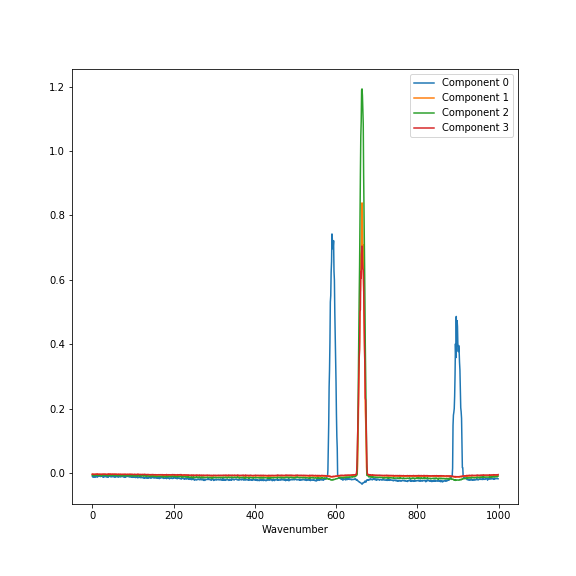
\includegraphics[width=0.5\textwidth]{figures/raman_sim_3_encode_layer_1_finetune_13.png}
\end{figure}


\begin{figure}
  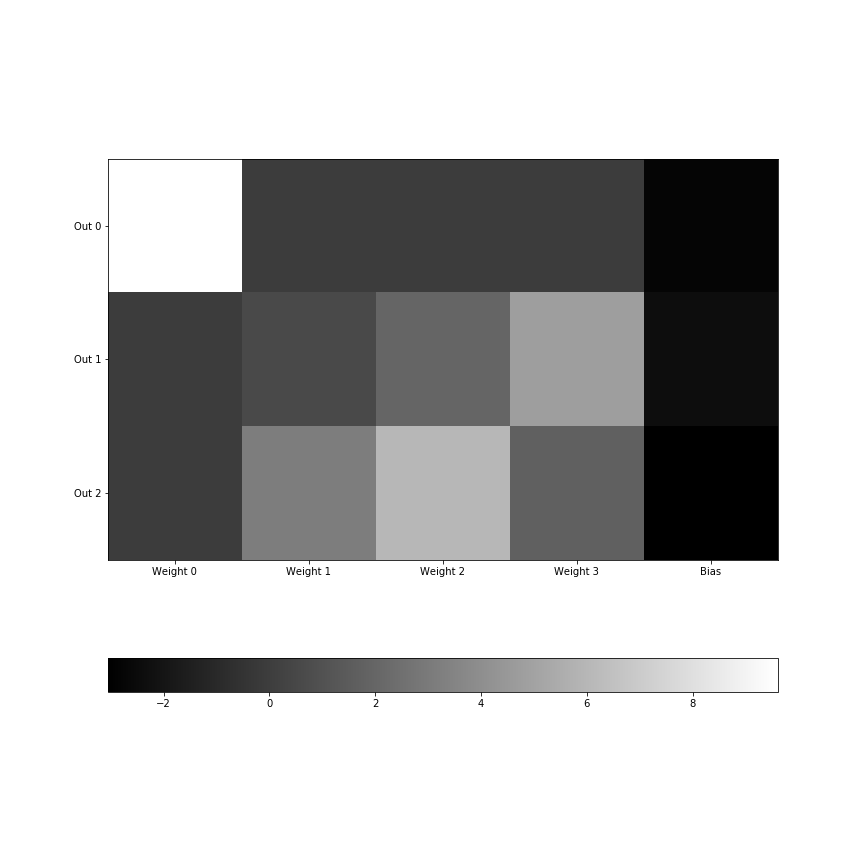
\includegraphics[width=0.23\textwidth]{figures/raman_sim_3_encode_layer_2_finetune_13.png}
  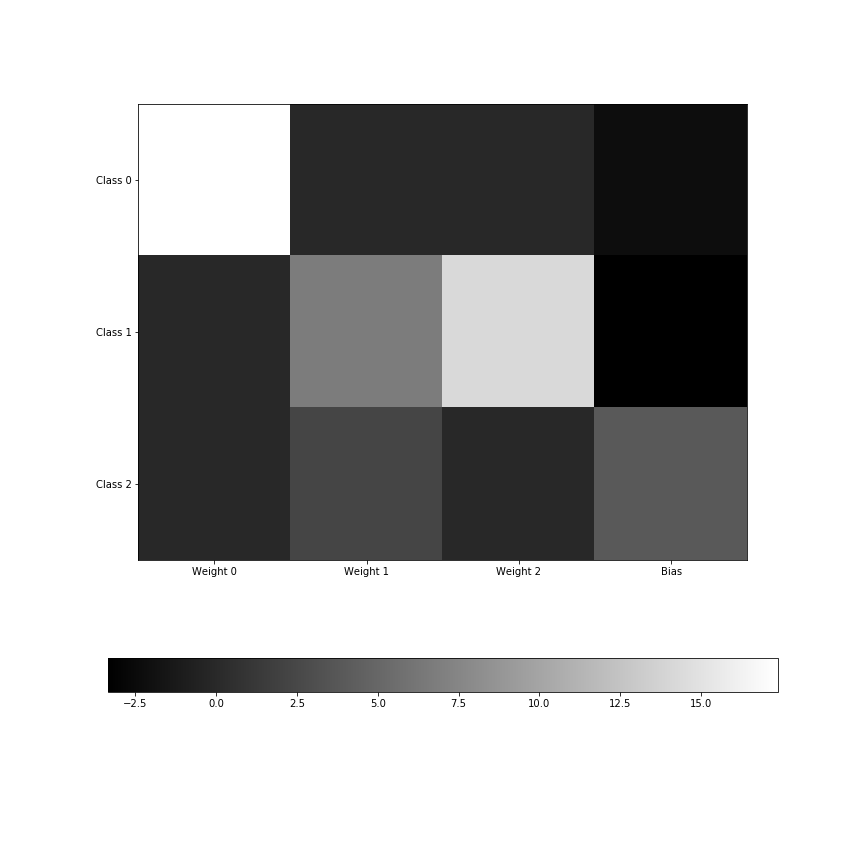
\includegraphics[width=0.23\textwidth]{figures/raman_sim_3_encode_layer_3_finetune_13.png}
\end{figure}


\begin{figure}
  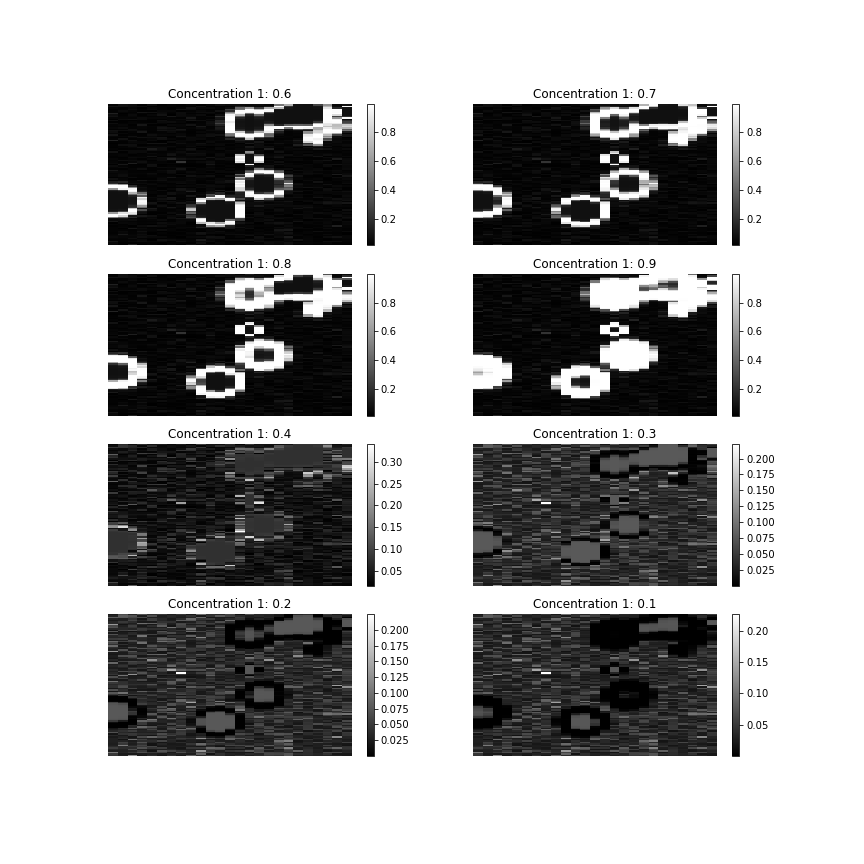
\includegraphics[width=0.30\linewidth]{figures/prop_substance_1_im.png}
  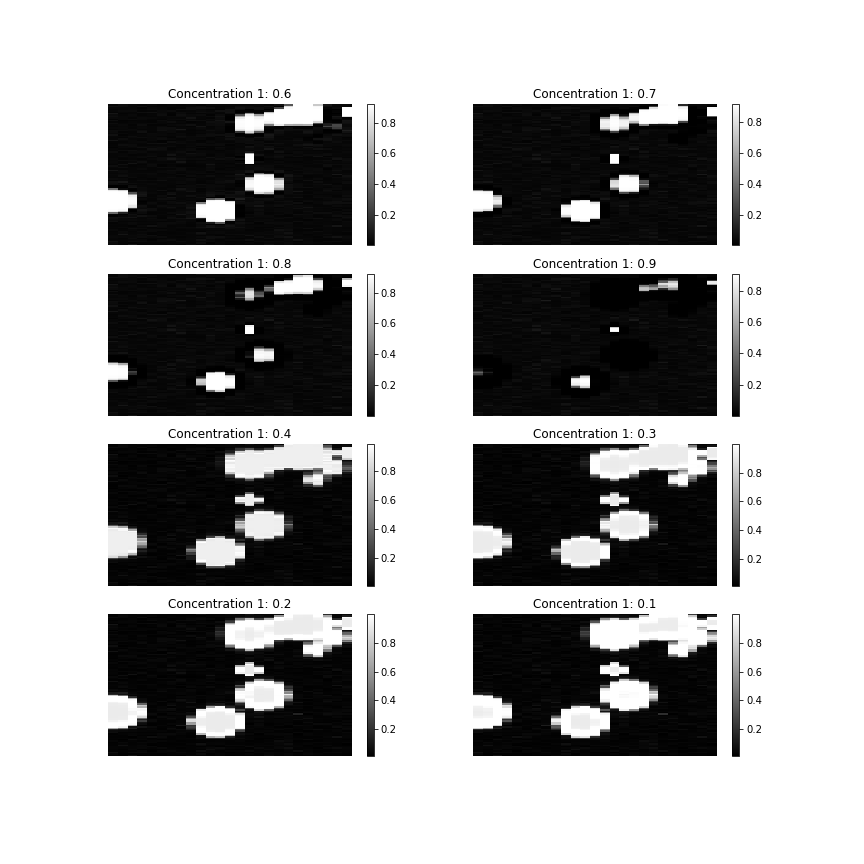
\includegraphics[width=0.30\linewidth]{figures/prop_substance_2_im.png}
  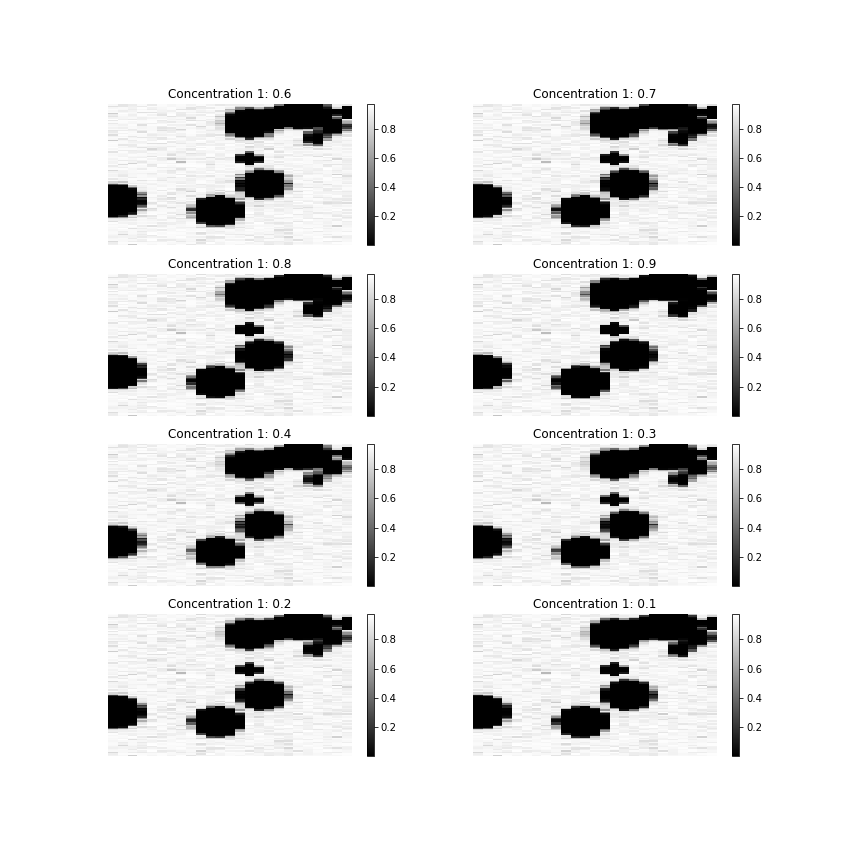
\includegraphics[width=0.30\linewidth]{figures/prop_substance_3_im.png}
\end{figure}



\begin{figure}
  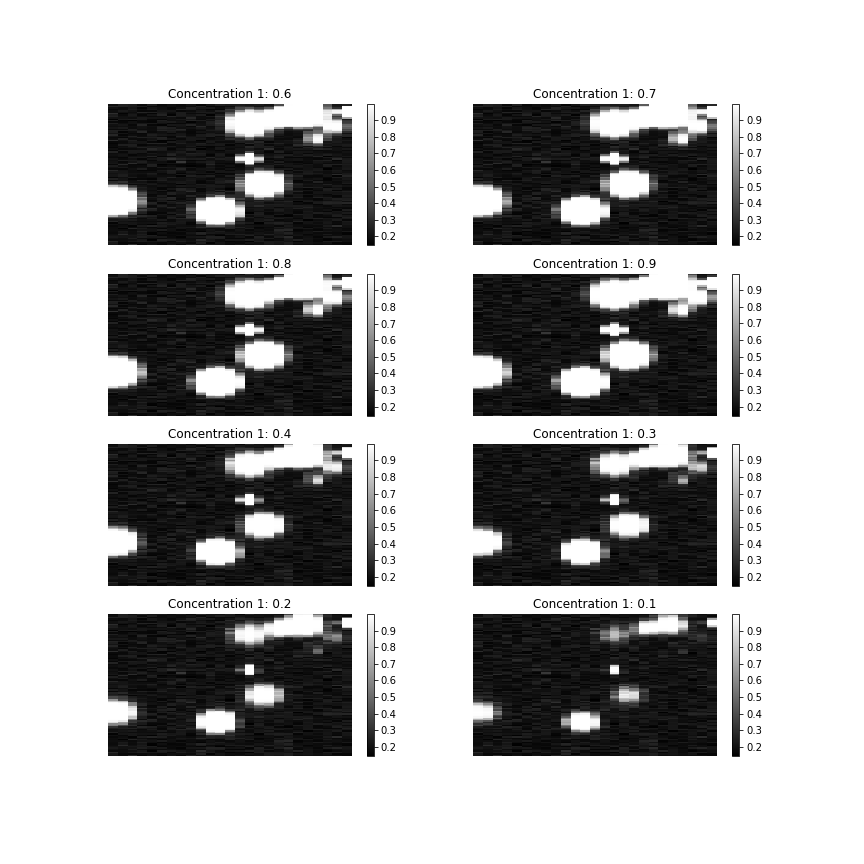
\includegraphics[width=0.30\linewidth]{figures/sigmoid_1_im.png}
  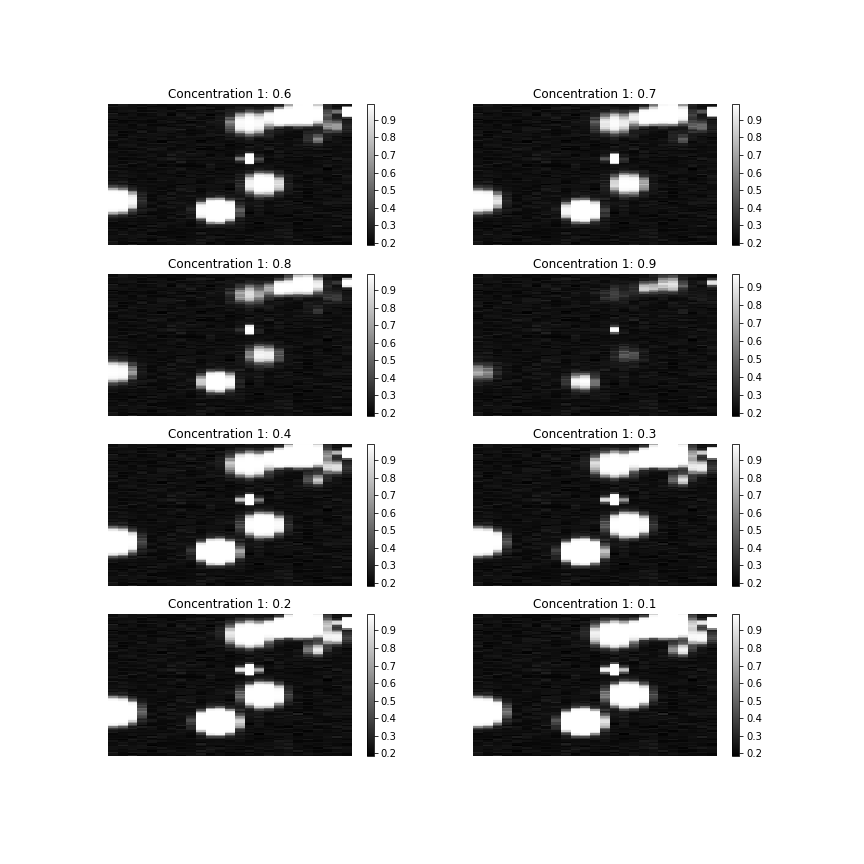
\includegraphics[width=0.30\linewidth]{figures/sigmoid_2_im.png}
  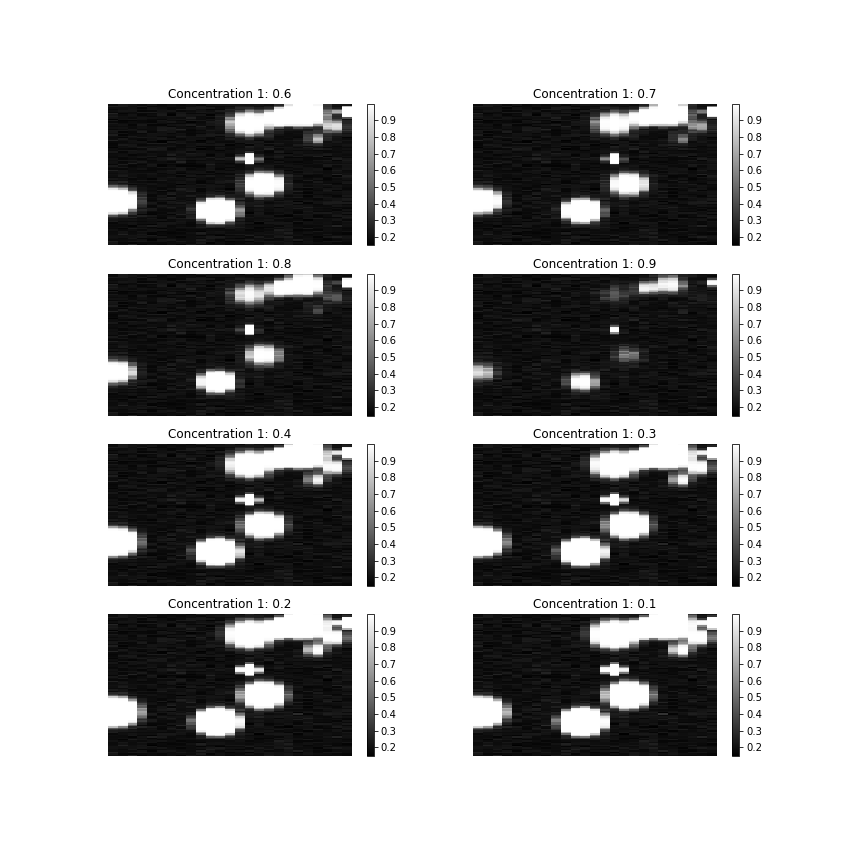
\includegraphics[width=0.30\linewidth]{figures/sigmoid_3_im.png}
\end{figure}



Classifier results


\begin{figure}
  
  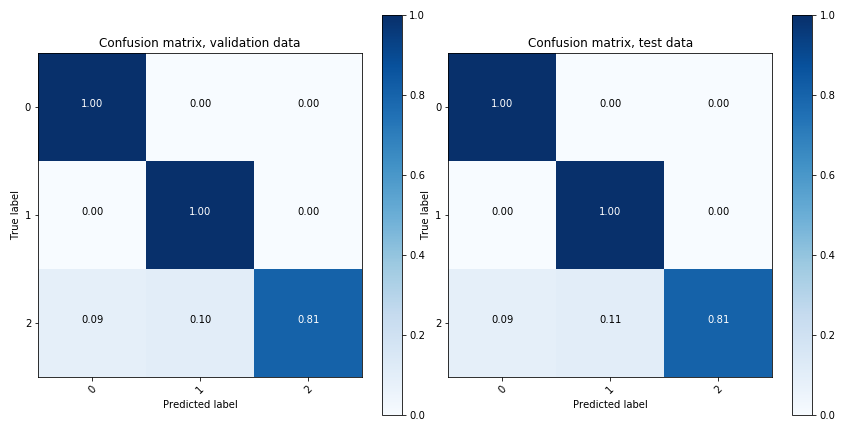
\includegraphics[width=0.5\textwidth]{figures/raman_sim_3_conf_matrix13.png}

\end{figure}

\section{Discussion}
\label{sec:discussion}


\begin{figure}
  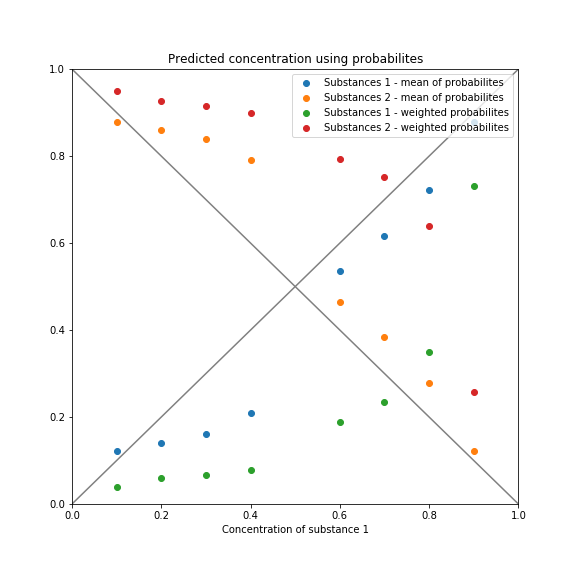
\includegraphics[width=0.23\textwidth]{figures/DNN_pred_conc_prob.png}
  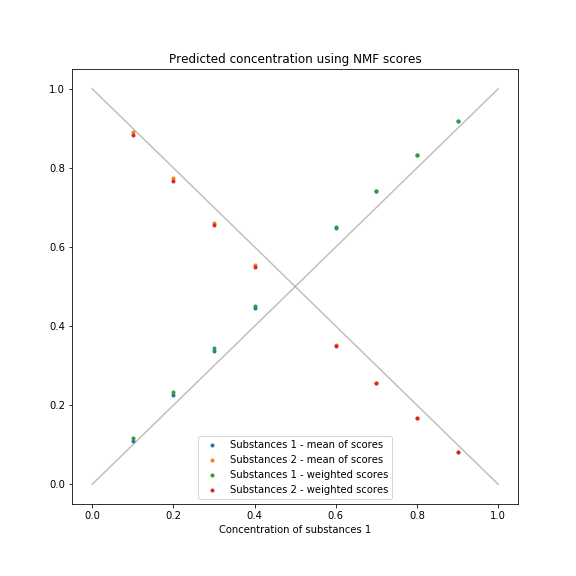
\includegraphics[width=0.23\textwidth]{figures/nmf_pred_conc.png}
\end{figure}

Comparison with NMF

\section{Conclusion}
\label{ssec:conclusion}


% Below is an example of how to insert images. Delete the ``\vspace'' line,
% uncomment the preceding line ``\centerline...'' and replace ``imageX.ps''
% with a suitable PostScript file name.

% To start a new column (but not a new page) and help balance the last-page
% column length use \vfill\pagebreak.
% -------------------------------------------------------------------------
\vfill
\pagebreak



\section{REFERENCES}
\label{sec:ref}

List and number all bibliographical references at the end of the paper.  The references can be numbered in alphabetic order or in order of appearance in the document.  When referring to them in the text, type the corresponding reference number in square brackets as shown at the end of this sentence .

% References should be produced using the bibtex program from suitable
% BiBTeX files (here: strings, refs, manuals). The IEEEbib.bst bibliography
% style file from IEEE produces unsorted bibliography list.
% -------------------------------------------------------------------------
\bibliographystyle{IEEEbib}
\bibliography{mendeley}

\end{document}
